


\documentclass [12pt]{article}

\title{Evaluating The Quality Of Signal Operations Using Automated Traffic Signal Performance Measures}
\author{Bangyu(Bruce) Wang\\Brigham Young University}

\usepackage{graphicx}
\usepackage{natbib}
\usepackage{float}
\begin{document}
\maketitle
\nocite{*}

\section{Literature Review}
A literature review was performed to gain insight and understanding on Automated Traffic Signal Performance Measures (ATSPM) evaluation as well as methods utilized in other industries for evaluating performance measures\cite{day2014performance}. This chapter contains a summary of that literature review with discussion provided on several key topics.  First, ATSPMs will be defined and the current practices for using ATSPMs will be explained. Second, each performance measure and evaluation tool currently used by the Utah Department of Transportation (UDOT) will be described. Third, the effects of ATSPMs on intersection and corridor performance will be discussed. Finally, methods for evaluating signal performance measures will be summarized\cite{day2018data}.

\section{Performance Measures Used Currently by the Utah Department of Transportation}
This section will summarize the performance measures and tools for visualizing and evaluating performance measures that UDOT currently uses in their ATSPM system Including the Purdue Phase Termination diagram, Split Monitor, Pedestrian Delay, Preemption Details, Turning Movement Counts, PCD, Approach Volume, Approach Delay, Arrivals on Red, Approach Speed, Yellow and Red Actuations, and Purdue Split Failure.

\begin{table}[ht]
    \centering
    \begin{tabular}{|p{6cm}|p{6cm}|}
    \hline
    Detection & Metric \\
    \hline
    None & Phase Termination Chart \newline Split Monitor \newline Preemption Details \newline Pedestrian Delay \\
    \hline
    Lane-by-lane Presence \newline Lane Group Presence & Purdue Split Failure \\
    \hline
    Lane-by-lane \newline Stop Bar Count & Turning Movement Counts \newline Approach Volume \\
    \hline
    Advanced Count & Purdue Coordination Diagram \newline Approach Volume \\
    \hline
    Advanced Speed & Approach Speed \\
    \hline
    \end{tabular}
    \caption{UDOT detection and metrics}
    \label{tab:my_label}
\end{table}

\subsection{Purdue Phase Termination}
This section will summarize the performance measures and tools for visualizing and evaluating performance measures that UDOT currently uses in their ATSPM system Including the Purdue Phase Termination diagram, Split Monitor, Pedestrian Delay, Preemption Details, Turning Movement Counts, PCD, Approach Volume, Approach Delay, Arrivals on Red, Approach Speed, Yellow and Red Actuations, and Purdue Split Failure.

\subsection{Methodology Equations}

This section shows the methodology equation used in this research. The percent on green (POG) can be used to determine the platoon ratio (Rp). The formula is \ref{PlatoonRatio} 

\begin{equation}
    Rp = POG/(g/C)
    \label{PlatoonRatio}
\end{equation}

\begin{figure}[ht]
    \centering
    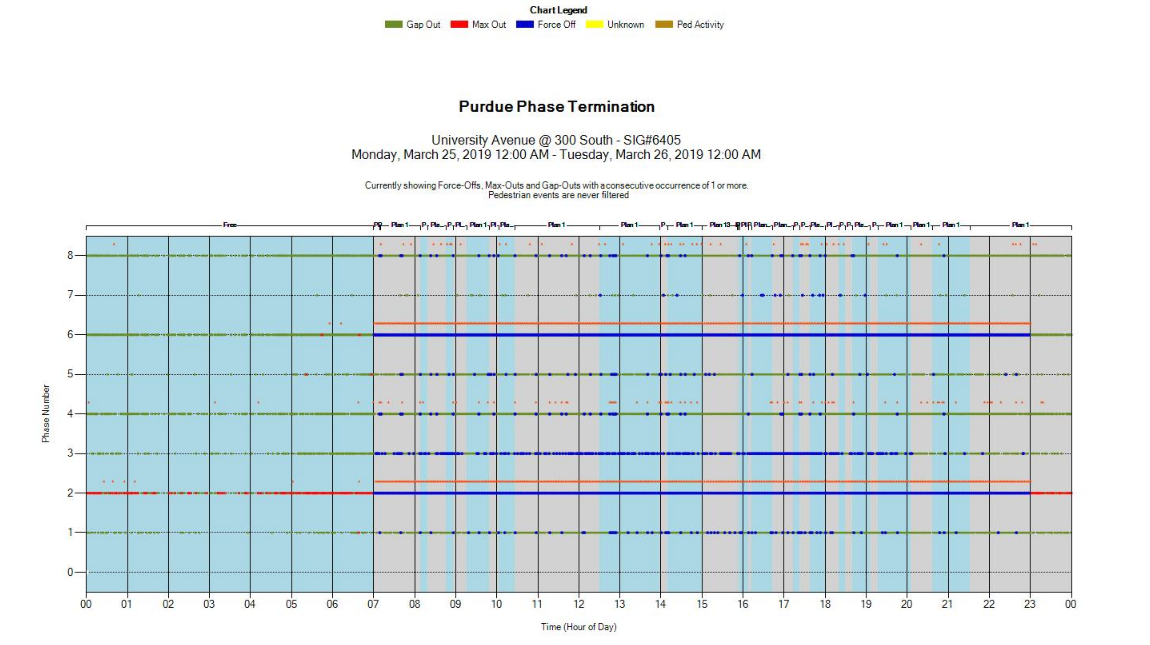
\includegraphics[height=3in]{1.png}
    \caption{Purdue Phase Termination diagram for 300 South and University Avenue in Provo, Utah}
    \label{fig:my_label}
\end{figure}





\bibliography{HW2}
\bibliographystyle{plain}
\end{document}